%%%%%%%%%%%%%%%%%%%%%%%%%%%%%%%%%%%%%%%%% 
% Beamer Presentation
% LaTeX Template
% Version 1.0 (10/11/12)
% 
% This template has been downloaded from:
% http://www.LaTeXTemplates.com
% 
% License:
% CC BY-NC-SA 3.0 (http://creativecommons.org/licenses/by-nc-sa/3.0/)
% 
%%%%%%%%%%%%%%%%%%%%%%%%%%%%%%%%%%%%%%%%% 

% ----------------------------------------------------------------------------------------
%	PACKAGES AND THEMES
% ----------------------------------------------------------------------------------------

\documentclass{beamer}

\mode<presentation> {

  % The Beamer class comes with a number of default slide themes
  % which change the colors and layouts of slides. Below this is a list
  % of all the themes, uncomment each in turn to see what they look like.

  % \usetheme{default}
  % \usetheme{AnnArbor}
  % \usetheme{Antibes}
  % \usetheme{Bergen}
  % \usetheme{Berkeley}
  % \usetheme{Berlin}
  % \usetheme{Boadilla}
  % \usetheme{CambridgeUS}
  % \usetheme{Copenhagen}
  % \usetheme{Darmstadt}
  % \usetheme{Dresden}
  % \usetheme{Frankfurt}
  % \usetheme{Goettingen}
  % \usetheme{Hannover}
  % \usetheme{Ilmenau}
  % \usetheme{JuanLesPins}
  % \usetheme{Luebeck}
  \usetheme{Madrid}
  % \usetheme{Malmoe}
  % \usetheme{Marburg}
  % \usetheme{Montpellier}
  % \usetheme{PaloAlto}
  % \usetheme{Pittsburgh}
  % \usetheme{Rochester}
  % \usetheme{Singapore}
  % \usetheme{Szeged}
  % \usetheme{Warsaw}

  % As well as themes, the Beamer class has a number of color themes
  % for any slide theme. Uncomment each of these in turn to see how it
  % changes the colors of your current slide theme.

  % \usecolortheme{albatross}
  % \usecolortheme{beaver}
  % \usecolortheme{beetle}
  % \usecolortheme{crane}
  % \usecolortheme{dolphin}
  % \usecolortheme{dove}
  % \usecolortheme{fly}
  % \usecolortheme{lily}
  % \usecolortheme{orchid}
  % \usecolortheme{rose}
  % \usecolortheme{seagull}
  % \usecolortheme{seahorse}
  % \usecolortheme{whale}
  % \usecolortheme{wolverine}

  % \setbeamertemplate{footline} % To remove the footer line in all slides uncomment this line
  % \setbeamertemplate{footline}[page number] % To replace the footer line in all slides with a simple slide count uncomment this line

  % \setbeamertemplate{navigation symbols}{} % To remove the navigation symbols from the bottom of all slides uncomment this line
}

\usepackage{hyperref}
\newcommand{\myhref}[3][blue]{\href{#2}{\texttt{\color{#1}{#3}}}}%
\usepackage{array}
\usepackage{amsmath}
\usepackage{tikz}
\usetikzlibrary{decorations}
% \renewcommand{\familydefault}{\rmdefault}
% \usepackage[scaled=1]{helvet}
% \usepackage[helvet]{sfmath}
% \everymath={\sf}
\usepackage{lmodern}
\newcolumntype{L}[1]{>{\raggedright\let\newline\\\arraybackslash\hspace{0pt}}m{#1}}
\newcolumntype{C}[1]{>{\centering\let\newline\\\arraybackslash\hspace{0pt}}m{#1}}
\newcolumntype{R}[1]{>{\raggedleft\let\newline\\\arraybackslash\hspace{0pt}}m{#1}}
\newcommand{\mb}[1]{\mathbf{#1}}
\rmfamily
\usefonttheme[onlymath]{serif}
\usepackage{graphicx} % Allows including images
\usepackage{booktabs} % Allows the use of \toprule, \midrule and \bottomrule in tables
\usepackage{subcaption}
\definecolor{bleu_cite}{RGB}{12,127,172}
\usepackage[style=bwl-FU,backend=bibtex]{biblatex}
\addbibresource{ref.bib}
\AtEveryCite{\color{bleu_cite}}
% ----------------------------------------------------------------------------------------
%	TITLE PAGE 
% ----------------------------------------------------------------------------------------

\title[A Bayesian Perspective of Neural Networks]{A Bayesian Perspective of Neural Networks} % The short title appears at the bottom of every slide, the full title is only on the title page

\author{Ethan Goan} % Your name
\institute[QUT] % Your institution as it will appear on the bottom of every slide, may be shorthand to save space
{
  Supervised by\\
  Prof. Clinton Fookes, Dr. Dimitri Perrin and Prof. Kerrie Mengersen\\
  \vspace*{3cm}
  
\includegraphics[scale=0.3]{figs/qut.eps}\\
  Queensland University of Technology \\ % Your institution for the title page
  \medskip
}
\date{} % Date, can be changed to a custom date
\begin{document}

\begin{frame}
  \titlepage % Print the title page as the first slide
\end{frame}

% ----------------------------------------------------------------------------------------
%	PRESENTATION SLIDES
% ----------------------------------------------------------------------------------------

% ------------------------------------------------
\section{First Section} % Sections can b % Your email addresse created in order to organize your presentation into discrete blocks, all sections and subsections are automatically printed in the table of contents as an overview of the talk
% ------------------------------------------------

\subsection{Subsection Example} % A subsection can be created just before a set of slides with a common theme to further break down your presentation into chunks
% 
% 
% 
% 
% ------------------------------------------------
\begin{frame}
  \frametitle{Overview}
  \begin{itemize}
  \item Introduce Neural Networks
  \item Some examples of neural networks applied to regression tasks
  \item Comparison to probabilistic models
  \item Recent research in the field of Bayesian Neural Networks
  \end{itemize}
\end{frame}
% 
% 
% 
% 
% ------------------------------------------------

% ------------------------------------------------

\begin{frame}
  \frametitle{Neural Network Graphical Model}
  \tikzset{%
  neuron missing/.style={
    draw=none, 
    scale=4,
    text height=0.333cm,
    execute at begin node=\color{black}$\vdots$
  },
}

\hspace*{1.5cm}
\begin{tikzpicture}[x=1.5cm, y=1.5cm, >=stealth]
  % draw input features  
  \foreach \m/\l [count=\y] in {1,2,3}
  {
    \node [circle,fill=green!50,minimum size=1cm] (input-\m) at (0,2.5-\y) {};
  }
  \foreach \m/\l [count=\y] in {4}
  {
    \node [circle,fill=green!50,minimum size=1cm ] (input-\m) at (0,-2.5) {};
  }
  
  \node [neuron missing]  at (0,-1.5) {};

  \foreach \m [count=\y] in {1}
  \node [circle,fill=red!50,minimum size=1cm ] (hidden-\m) at (2,0.75) {};

  % draw hidden layers
  \foreach \m [count=\y] in {2}
  \node [circle,fill=red!50,minimum size=1cm ] (hidden-\m) at (2,-1.85) {};  
  \node [neuron missing]  at (2,-0.3) {};

  % draw output neurons
  \foreach \m [count=\y] in {1}
  \node [circle,fill=blue!50,minimum size=1cm ] (output-\m) at (4,0.5-\y) {};

  \foreach \l [count=\i] in {1,2,3,n_x}
  \draw [<-] (input-\i) -- ++(-1,0)
  node [above, midway] {$x_{\l}$};
  \foreach \l [count=\i] in {1}
  \node [above] at (input-\i.north) {$\vec{x}$};

  
  \foreach \l [count=\i] in {1,k}
  \node [above] at (hidden-\i.north) {$H^{[l]}_{\l}$};

  \draw [->] (output-1) -- ++(1,0)
  node [above, midway] {$O_{1}$};

  \foreach \i in {1,...,4}
  \foreach \j in {1,...,2}
  \draw [->] (input-\i) -- (hidden-\j);

  \foreach \i in {1,...,2}
  \draw [->] (hidden-\i) -- (output-1);

  % \foreach \l [count=\x from 0] in {Input, Hidden, Ouput}
  % \node [align=center, above] at (\x*2,2) {\l \\ layer};

\end{tikzpicture}

\end{frame}
% 
% 
% 
% 
% ------------------------------------------------
\begin{frame}
  \frametitle{Inside a Neuron}
  Neuron consists of a linear mapping of the input, followed by a non-linear activation.
  \begin{align*}
    a^{[i]}_j &= g( \mb{w}^{[i]T}_j \mb{x} + b^{[i]}_j) 
    \\
    \mb{w}^{[i]T}_j &= \text{ weight vector}
    \\
    b^{[i]T}_j  &= \text{ bias}
    \\
    g( \cdot ) &= \text{ non-linear activation function}
    \\
    [i] &= \text{ layer number}
    \\
    j &= \text{ node number within the } i^{th} \text{ layer}
  \end{align*}
  % 
  % 
  % 
  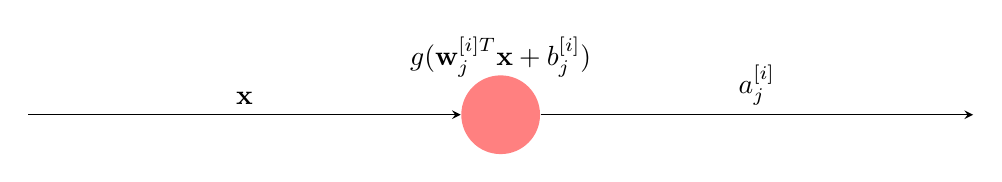
\begin{tikzpicture}[x=1.5cm, y=2.5cm,>=stealth]
    \centering
    \node[circle,fill=red!50,minimum size=1cm] at (0,0) (hidden) {} ;
    \draw [<-] (hidden) -- ++(-4,0)
    node [above, midway] {$\mb{x}$};
    \node [above=10] at (hidden) {$g( \mb{w}^{[i]T}_j \mb{x} + b^{[i]}_j)$};
    \draw [->] (hidden) -- ++(4,0)
    node [above, midway=-10] {$a^{[i]}_j$};
  \end{tikzpicture}
\end{frame}
% 
% 
% 
% 
% ------------------------------------------------
\begin{frame}
  \frametitle{Vectorisation}
  Can implement the neural network model more efficiently by using matrix operations.
  \begin{equation*}
    \mathbf{z}^{[1]} = W^{[1]}\mathbf{x} + \mathbf{b}^{[1]} = 
    \begin{bmatrix}
      \cdots & w_{1}^{[1]T} & \cdots \\
      \cdots & w_{2}^{[1]T} & \cdots \\
      & \vdots       &  \\
      \cdots & w_{k_l}^{[1]T} & \cdots \\
    \end{bmatrix}
    \begin{bmatrix}
      x_1\\
      x_2\\
      \vdots\\
      x_{n_x}
    \end{bmatrix}
    + 
    \begin{bmatrix}
      b_{1}^{[1]} \\
      b_{2}^{[1]} \\
      \vdots \\
      b_{k_l}^{[1]} \\
    \end{bmatrix}
  \end{equation*}
  % 
  % 
  \vspace*{1cm}
  % 
  % 
  \begin{equation*}
    \mb{a}^{[1]} = g( \mb{z}^{[1]} )
  \end{equation*}
\end{frame}
% 
% 
% 
% 
% ------------------------------------------------
\begin{frame}
  \frametitle{Further Vectorisation - Multiple Input Vectors}
  Can pass all (or as much as physically possible) into the network in a single iteration by storing the input vectors $\mb{x}_i$ as columns of a matrix $X$.
  \begin{equation*}
    Z^{[1]} = W^{[1]} X + \mathbf{b}^{[1]} = 
    \begin{bmatrix}
      \cdots & w_{1}^{[1]T} & \cdots \\
      \cdots & w_{2}^{[1]T} & \cdots \\
      & \vdots       &  \\
      \cdots & w_{k_l}^{[1]T} & \cdots \\
    \end{bmatrix}
    \begin{bmatrix}
      \vdots & \vdots & & \vdots\\
      \mathbf{x}^{(1)} & \mathbf{x}^{(2)} &  \cdots & \mathbf{x}^{(m)}\\
      \vdots & \vdots & & \vdots\\
    \end{bmatrix}
    + 
    \begin{bmatrix}
      b_{1}^{[1]} \\
      b_{2}^{[1]} \\
      \vdots \\
      b_{k_l}^{[1]} \\
    \end{bmatrix}
  \end{equation*}
  % 
  % 
  \vspace*{1cm}
  % 
  % 
  \begin{equation*}
    A^{[1]} = g( Z^{[1]} )
  \end{equation*}
\end{frame}
% 
% 
% 
% 
% ------------------------------------------------
\begin{frame}
  \frametitle{Training - Gradient Descent}
  Forward Propagation in a 2 layer network (1 hidden layer)
  \begin{align*}
    Z^{[1]} &= W^{[1]}X + b^{[1]}\\
    A^{[1]} &= g(Z^{[1]})\\
    Z^{[2]} &= W^{[2]}A^{[1]} + b^{[2]}\\
    A^{[2]} &= g(Z^{[2]}) = \hat{y}
  \end{align*}
  % 
  % 
  To perform gradient descent, first need to define an objective to minimise.
  \begin{equation*}
    \mathcal{L}(\hat{y}, y) = - \Big(y\log(\hat{y}) + (1-y)\log(1 - \hat{y})  \Big)
  \end{equation*}
  \begin{equation*}
    J(w,b) =\frac{1}{m} \Sigma_{i=1}^{m}\mathcal{L}(\hat{y}_i, y_i)
  \end{equation*}
\end{frame}
% 
% 
% 
% 
% ------------------------------------------------
\begin{frame}
  \frametitle{Training - Gradient Descent}
  With our cost objective to minimise,
  \begin{equation*}
    J(w,b) =\frac{1}{m} \Sigma_{i=1}^{m}\mathcal{L}(\hat{y}_i, y_i)
  \end{equation*}
  we can find the partial derivative of this objective and use it to update out network parameters.
  \begin{equation*}
    \theta = \theta - \alpha \dfrac{\partial J}{\partial \theta}
  \end{equation*}
  where $\alpha$ is our learning rate, and $\theta$ is any of our model weights $W^{[l]}$ or bias' $\mb{b}^{[l]}$.
\end{frame}
% 
% 
% 
% 
% ------------------------------------------------
\begin{frame}
  \frametitle{More Hidden Layers}
  \tikzset{%
  neuron missing/.style={
    draw=none, 
    scale=4,
    text height=0.333cm,
    execute at begin node=\color{black}$\vdots$
  },
}

\tikzset{%
  neuron horizontal/.style={
    draw=none, 
    scale=4,
    text height=0.333cm,
    execute at begin node=\color{black}$\cdots$
  },
}


\hspace*{0.75cm}
\begin{tikzpicture}[x=1.5cm, y=1.5cm, >=stealth]
  % draw input features  
  \foreach \m/\l [count=\y] in {1,2,3}
  {
    \node [circle,fill=green!50,minimum size=1cm] (input-\m) at (0,2.5-\y) {};
  }
  \foreach \m/\l [count=\y] in {4}
  {
    \node [circle,fill=green!50,minimum size=1cm ] (input-\m) at (0,-2.5) {};
  }

  % draw hidden layers
  % first layer
  \node [neuron missing]  at (0,-1.5) {};

  \foreach \m [count=\y] in {1}
  \node [circle,fill=red!50,minimum size=1cm ] (hidden1-\m) at (2,0.75) {};

  \foreach \m [count=\y] in {2}
  \node [circle,fill=red!50,minimum size=1cm ] (hidden1-\m) at (2.0,-1.85) {};  
  \node [neuron missing]  at (2,-0.3) {};

  % second layer
  \node [neuron missing]  at (3.5,-0.3) {};
  \foreach \m [count=\y] in {1}
  \node [circle,fill=red!50,minimum size=1cm ] (hidden2-\m) at (3.5, 0.75) {};

  
  \foreach \m [count=\y] in {2}
  \node [circle,fill=red!50,minimum size=1cm ] (hidden2-\m) at (3.5,-1.85) {};  
  \node [neuron missing]  at (2,-0.3) {};
  
  % draw output neuron
  \foreach \m [count=\y] in {1}
  \node [circle,fill=blue!50,minimum size=1cm ] (output-\m) at (5.0,0.5-\y) {};

  \foreach \l [count=\i] in {1}
  \node [above] at (input-\i.north) {$\vec{x}$};

  \foreach \l [count=\i] in {1,2,3,n_x}
  \draw [<-] (input-\i) -- ++(-1,0)
  node [above, midway] {$x_{\l}$};

  \foreach \l [count=\i] in {1,k_1}
  \node [above] at (hidden1-\i.north) {$H^{[1]}_{\l}$};

  \foreach \l [count=\i] in {1,k_l}
  \node [above] at (hidden2-\i.north) {$H^{[l]}_{\l}$};

  \draw [->] (output-1) -- ++(1,0)
  node [above, midway] {$O_{1}$};

  \foreach \i in {1,...,4}
  \foreach \j in {1,...,2}
  \draw [->] (input-\i) -- (hidden-\j);

  \foreach \i in {1,...,2}
  \foreach \j in {1,...,2}
  \draw [->] (hidden1-\i) -- (hidden2-\j);

  \foreach \i in {1,...,2}
  \draw [->] (hidden2-\i) -- (output-1);
  
  % \foreach \l [count=\x from 0] in {Input, Hidden, Ouput}
  % \node [align=center, above] at (\x*2,2) {\l \\ layer};

\end{tikzpicture}

\end{frame}
% 
% 
% 
% 
% ------------------------------------------------
\begin{frame}
  \frametitle{Comparison - Regression}
  \vspace*{-0.15cm}
  \begin{figure}[!h]
    \centering
    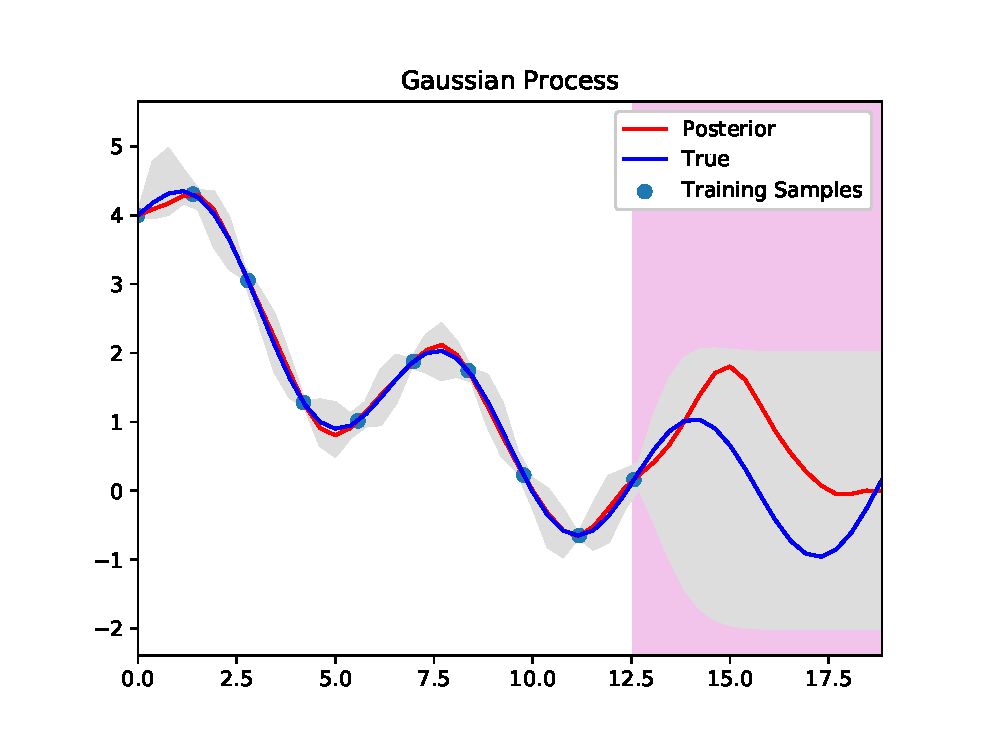
\includegraphics[width=0.8\linewidth]{./figs/gp.eps}
    \caption{Regression using Gaussian Process}
    \label{fig:gp}
  \end{figure}
\end{frame}
% 
% 
% 
% 
% ------------------------------------------------
\begin{frame}
  \frametitle{Comparison - Regression}
  \vspace*{-0.15cm}
  \begin{figure}[!h]
    \centering
    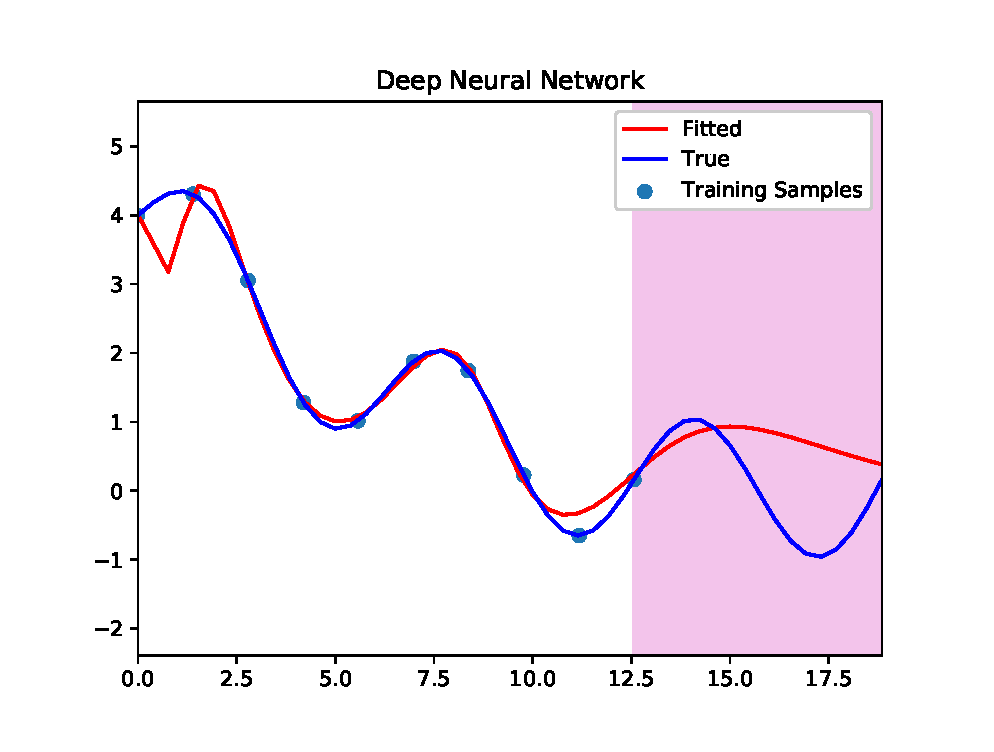
\includegraphics[width=0.8\linewidth]{./figs/nn.eps}
    \caption{Regression using neural network with two hidden layers}
    \label{fig:nn}
  \end{figure}
\end{frame}
% 
% 
% 
% 
% ------------------------------------------------
\begin{frame}
  \frametitle{Stochastic Regularisation Techniques}
  \begin{itemize}
  \item Neural networks are prone to overfitting training data
  \item Stochastic Regularisation Techniques (SRTs) are introduced to combat this
  \item Most prominent technique is Dropout, where output of a unit is attenuated by multiplying element with a Bernoulli distributed RV \cite{sriv2014}
  \end{itemize}
\end{frame}
% 
% 
%
\begin{frame}
  \frametitle{Dropout}
  With dropout, the feedforward opertation becomes,
  \begin{align*}
    r_j^{[i]} & \sim \textrm{Bernoulli}(p)\\
    R^{[i]} &= \textrm{diag}(\mb{\epsilon})\\
    \widetilde{A}^{[i-1]} &= R^{[i]}A^{[i-1]} \\
    \widetilde{Z}^{[i]} &= W^{[i]}\widetilde{A}^{[i-1]} + b^{[i]}\\
    \widetilde{A}^{[i]} &= g(\widetilde{Z}^{[i]})\\
  \end{align*}    
\end{frame}
% 
% 
% ------------------------------------------------
\begin{frame}
  \frametitle{Before Applying Dropout}
  \pgfdeclaredecoration{discontinuity}{start}{
  \state{start}[width=0.5\pgfdecoratedinputsegmentremainingdistance-0.5\pgfdecorationsegmentlength,next state=first wave]
  {}
  \state{first wave}[width=\pgfdecorationsegmentlength, next state=second wave]
  {
    \pgfpathlineto{\pgfpointorigin}
    \pgfpathmoveto{\pgfqpoint{0pt}{\pgfdecorationsegmentamplitude}}
    \pgfpathcurveto
        {\pgfpoint{-0.25*\pgfmetadecorationsegmentlength}{0.75\pgfdecorationsegmentamplitude}}
        {\pgfpoint{-0.25*\pgfmetadecorationsegmentlength}{0.25\pgfdecorationsegmentamplitude}}
        {\pgfpoint{0pt}{0pt}}
    \pgfpathcurveto
        {\pgfpoint{0.25*\pgfmetadecorationsegmentlength}{-0.25\pgfdecorationsegmentamplitude}}
        {\pgfpoint{0.25*\pgfmetadecorationsegmentlength}{-0.75\pgfdecorationsegmentamplitude}}
        {\pgfpoint{0pt}{-\pgfdecorationsegmentamplitude}}
}
\state{second wave}[width=0pt, next state=do nothing]
  {
    \pgfpathmoveto{\pgfqpoint{0pt}{\pgfdecorationsegmentamplitude}}
    \pgfpathcurveto
        {\pgfpoint{-0.25*\pgfmetadecorationsegmentlength}{0.75\pgfdecorationsegmentamplitude}}
        {\pgfpoint{-0.25*\pgfmetadecorationsegmentlength}{0.25\pgfdecorationsegmentamplitude}}
        {\pgfpoint{0pt}{0pt}}
    \pgfpathcurveto
        {\pgfpoint{0.25*\pgfmetadecorationsegmentlength}{-0.25\pgfdecorationsegmentamplitude}}
        {\pgfpoint{0.25*\pgfmetadecorationsegmentlength}{-0.75\pgfdecorationsegmentamplitude}}
        {\pgfpoint{0pt}{-\pgfdecorationsegmentamplitude}}
    \pgfpathmoveto{\pgfpointorigin}
}
  \state{do nothing}[width=\pgfdecorationsegmentlength,next state=do nothing]{
    \pgfpathlineto{\pgfpointdecoratedinputsegmentlast}
  }
  \state{final}
  {
    \pgfpathlineto{\pgfpointdecoratedpathlast}
  }
}



\tikzset{%
  neuron missing/.style={
    draw=none, 
    scale=4,
    text height=0.333cm,
    execute at begin node=\color{black}$\vdots$
  },
}
\hspace*{1cm}
\begin{tikzpicture}[x=1.5cm, y=1.5cm, >=stealth]
  % draw input features  
  \foreach \m/\l [count=\y] in {1,2,3}
  {
    \node [circle,fill=green!50,minimum size=1cm] (input-\m) at (0,2.5-\y) {};
  }
  \foreach \m/\l [count=\y] in {4}
  {
    \node [circle,fill=green!50,minimum size=1cm ] (input-\m) at (0,-2.5) {};
  }
  
  \node [neuron missing]  at (0,-1.5) {};
  % draw hidden layers
  %first hidden layer
  \node [circle,fill=red!50,minimum size=1cm ] (hidden1-1) at (2,0.75) {};
  \node [circle,fill=red!50,minimum size=1cm ] (hidden1-2) at (2,-0.5) {};
  \node [circle,fill=red!50,minimum size=1cm ] (hidden1-3) at (2,-1.85) {};  
  %second hidden layer
  \node [circle,fill=red!50,minimum size=1cm ] (hidden2-1) at (3.5,0.75) {};
  \node [circle,fill=red!50,minimum size=1cm ] (hidden2-2) at (3.5,-0.5) {};
  \node [circle,fill=red!50,minimum size=1cm ] (hidden2-3) at (3.5,-1.85) {};  

  % draw output neurons
  \node [circle,fill=blue!50,minimum size=1cm ] (output-1) at (5,0.5) {};
  \node [circle,fill=blue!50,minimum size=1cm ] (output-2) at (5,-1.5) {};

  \foreach \l [count=\i] in {1}
  \node [above] at (input-\i.north) {$\vec{x}$};

  \foreach \l [count=\i] in {1,2,3,n_x}
  \draw [<-] (input-\i) -- ++(-1,0)
  node [above, midway] {$x_{\l}$};


  \draw [->] (output-1) -- ++(1,0)
  node [above, midway] {$O_{1}$};
  \draw [->] (output-2) -- ++(1,0)
  node [above, midway] {$O_{2}$};

  \foreach \i in {1,...,4}
  \foreach \j in {1,...,3}
  \draw [->] (input-\i) -- (hidden1-\j);

  \foreach \i in {1,2,3}
  \foreach \j in {1,2,3}
  \draw [->] (hidden1-\i) -- (hidden2-\j);
  
  \foreach \i in {1,2,3}
  \foreach \j in {1,2}
  \draw [->] (hidden2-\i) -- (output-\j);
  
  % \foreach \l [count=\x from 0] in {Input, Hidden, Ouput}
  % \node [align=center, above] at (\x*2,2) {\l \\ layer};

\end{tikzpicture}

\end{frame}
% 
% 
% 
% 
% ------------------------------------------------
\begin{frame}
  \frametitle{Example After Applying Dropout}
  \pgfdeclaredecoration{discontinuity}{start}{
  \state{start}[width=0.5\pgfdecoratedinputsegmentremainingdistance-0.5\pgfdecorationsegmentlength,next state=first wave]
  {}
  \state{first wave}[width=\pgfdecorationsegmentlength, next state=second wave]
  {
    \pgfpathlineto{\pgfpointorigin}
    \pgfpathmoveto{\pgfqpoint{0pt}{\pgfdecorationsegmentamplitude}}
    \pgfpathcurveto
        {\pgfpoint{-0.25*\pgfmetadecorationsegmentlength}{0.75\pgfdecorationsegmentamplitude}}
        {\pgfpoint{-0.25*\pgfmetadecorationsegmentlength}{0.25\pgfdecorationsegmentamplitude}}
        {\pgfpoint{0pt}{0pt}}
    \pgfpathcurveto
        {\pgfpoint{0.25*\pgfmetadecorationsegmentlength}{-0.25\pgfdecorationsegmentamplitude}}
        {\pgfpoint{0.25*\pgfmetadecorationsegmentlength}{-0.75\pgfdecorationsegmentamplitude}}
        {\pgfpoint{0pt}{-\pgfdecorationsegmentamplitude}}
}
\state{second wave}[width=0pt, next state=do nothing]
  {
    \pgfpathmoveto{\pgfqpoint{0pt}{\pgfdecorationsegmentamplitude}}
    \pgfpathcurveto
        {\pgfpoint{-0.25*\pgfmetadecorationsegmentlength}{0.75\pgfdecorationsegmentamplitude}}
        {\pgfpoint{-0.25*\pgfmetadecorationsegmentlength}{0.25\pgfdecorationsegmentamplitude}}
        {\pgfpoint{0pt}{0pt}}
    \pgfpathcurveto
        {\pgfpoint{0.25*\pgfmetadecorationsegmentlength}{-0.25\pgfdecorationsegmentamplitude}}
        {\pgfpoint{0.25*\pgfmetadecorationsegmentlength}{-0.75\pgfdecorationsegmentamplitude}}
        {\pgfpoint{0pt}{-\pgfdecorationsegmentamplitude}}
    \pgfpathmoveto{\pgfpointorigin}
}
  \state{do nothing}[width=\pgfdecorationsegmentlength,next state=do nothing]{
    \pgfpathlineto{\pgfpointdecoratedinputsegmentlast}
  }
  \state{final}
  {
    \pgfpathlineto{\pgfpointdecoratedpathlast}
  }
}



\tikzset{%
  neuron missing/.style={
    draw=none, 
    scale=4,
    text height=0.333cm,
    execute at begin node=\color{black}$\vdots$
  },
}
\hspace*{1cm}
\begin{tikzpicture}[x=1.5cm, y=1.5cm, >=stealth]
  % draw input features  
  \foreach \m/\l [count=\y] in {1,2,3}
  {
    \node [circle,fill=green!50,minimum size=1cm] (input-\m) at (0,2.5-\y) {};
  }
  \foreach \m/\l [count=\y] in {4}
  {
    \node [circle,fill=green!50,minimum size=1cm ] (input-\m) at (0,-2.5) {};
  }
  
  \node [neuron missing]  at (0,-1.5) {};
  % draw hidden layers
  %first hidden layer
  \node [circle,fill=red!50,minimum size=1cm ] (hidden1-1) at (2,0.75) {};
  \node [circle,fill=red!50,minimum size=1cm ] (hidden1-2) at (2,-0.5) {};
  \node [circle,fill=red!50,minimum size=1cm ] (hidden1-3) at (2,-1.85) {};  
  %second hidden layer
  \node [circle,fill=red!50,minimum size=1cm ] (hidden2-1) at (3.5,0.75) {};
  \node [circle,fill=red!50,minimum size=1cm ] (hidden2-2) at (3.5,-0.5) {};
  \node [circle,fill=red!50,minimum size=1cm ] (hidden2-3) at (3.5,-1.85) {};  

  % draw output neurons
  \node [circle,fill=blue!50,minimum size=1cm ] (output-1) at (5,0.5) {};
  \node [circle,fill=blue!50,minimum size=1cm ] (output-2) at (5,-1.5) {};

  \foreach \l [count=\i] in {1}
  \node [above] at (input-\i.north) {$\vec{x}$};

  \foreach \l [count=\i] in {1,2,3,n_x}
  \draw [<-] (input-\i) -- ++(-1,0)
  node [above, midway] {$x_{\l}$};


  \draw [->] (output-1) -- ++(1,0)
  node [above, midway] {$O_{1}$};
  \draw [->] (output-2) -- ++(1,0)
  node [above, midway] {$O_{2}$};

  \foreach \i in {1,...,4}
  \foreach \j in {1,...,3}
  \draw [->] (input-\i) -- (hidden1-\j);

  \foreach \i in {1,3}
  \foreach \j in {1,2,3}
  \draw [->] (hidden1-\i) -- (hidden2-\j);
  
  \foreach \i in {2,3}
  \foreach \j in {1,2}
  \draw [->] (hidden2-\i) -- (output-\j);
  
  % \foreach \l [count=\x from 0] in {Input, Hidden, Ouput}
  % \node [align=center, above] at (\x*2,2) {\l \\ layer};

\end{tikzpicture}

\end{frame}
% 
% 
% 
% 
% ------------------------------------------------


\begin{frame}
  \frametitle{A Bayesian Perspective}
  \begin{itemize}
  \item Want to relate neural networks to probabilistic methods
  \item Development of Bayesian Neural Networks (BNN)
  \item BNN is a neural network with a prior placed over the network parameters $W^{[i]}, \mb{b^{[i]}}$; \cite{tishby1989, Neal1996}
  \item Work in \cite{Neal1996} showed how when a Gaussian prior is placed over network parameters for a single hidden layer network, the prior on the network output is a Gaussian Process
  \end{itemize}
\end{frame}
% 
% 
% 
% 
% 
% ------------------------------------------------
\begin{frame}
  \frametitle{Gaussian Process Prior}
  \begin{figure}[!h]
    \centering
    \begin{subfigure}[b]{0.5\textwidth}
      \centering
      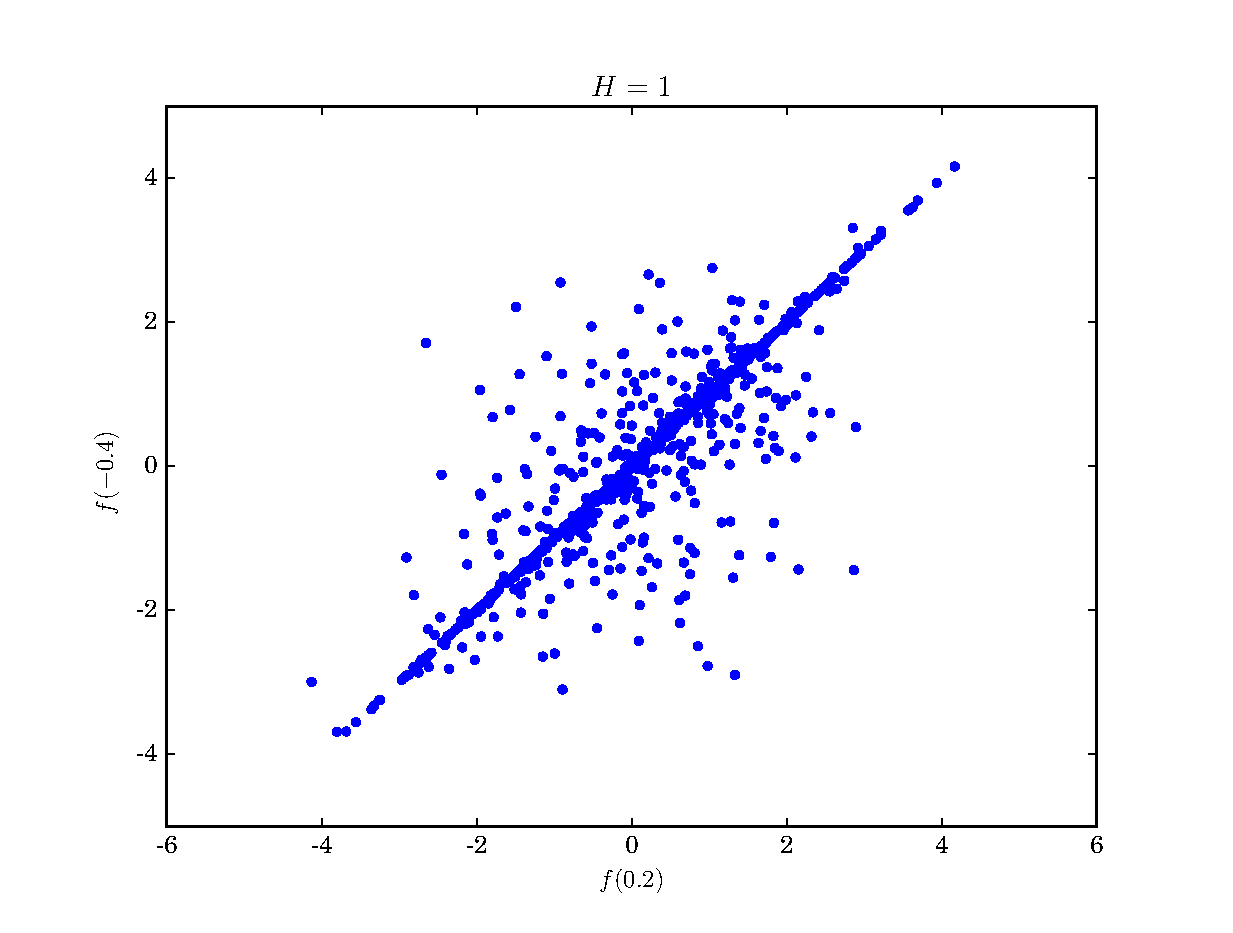
\includegraphics[width=\linewidth]{./figs/1.eps}
      \caption{1 hidden units}
    \end{subfigure}%
    ~ 
    \begin{subfigure}[b]{0.5\textwidth}
      \centering
      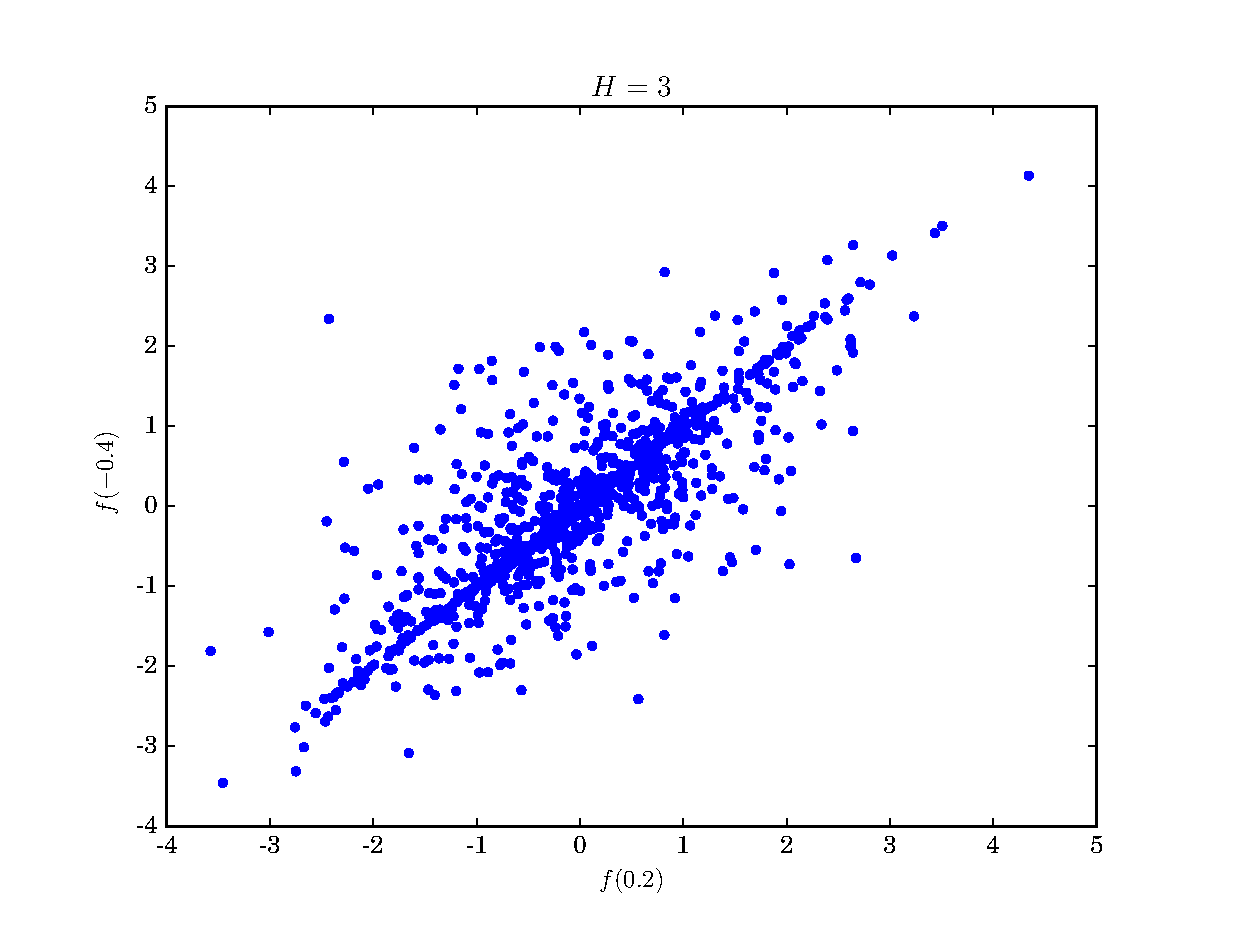
\includegraphics[width=\linewidth]{./figs/3.eps}
      \caption{3 hidden units}
    \end{subfigure}
  \end{figure}
\end{frame}
% 
% 
% 
% 
% ------------------------------------------------
\begin{frame}
  \frametitle{Gaussian Process Prior}
  \begin{figure}[!h]
    \centering
    \begin{subfigure}[b]{0.5\textwidth}
      \centering
      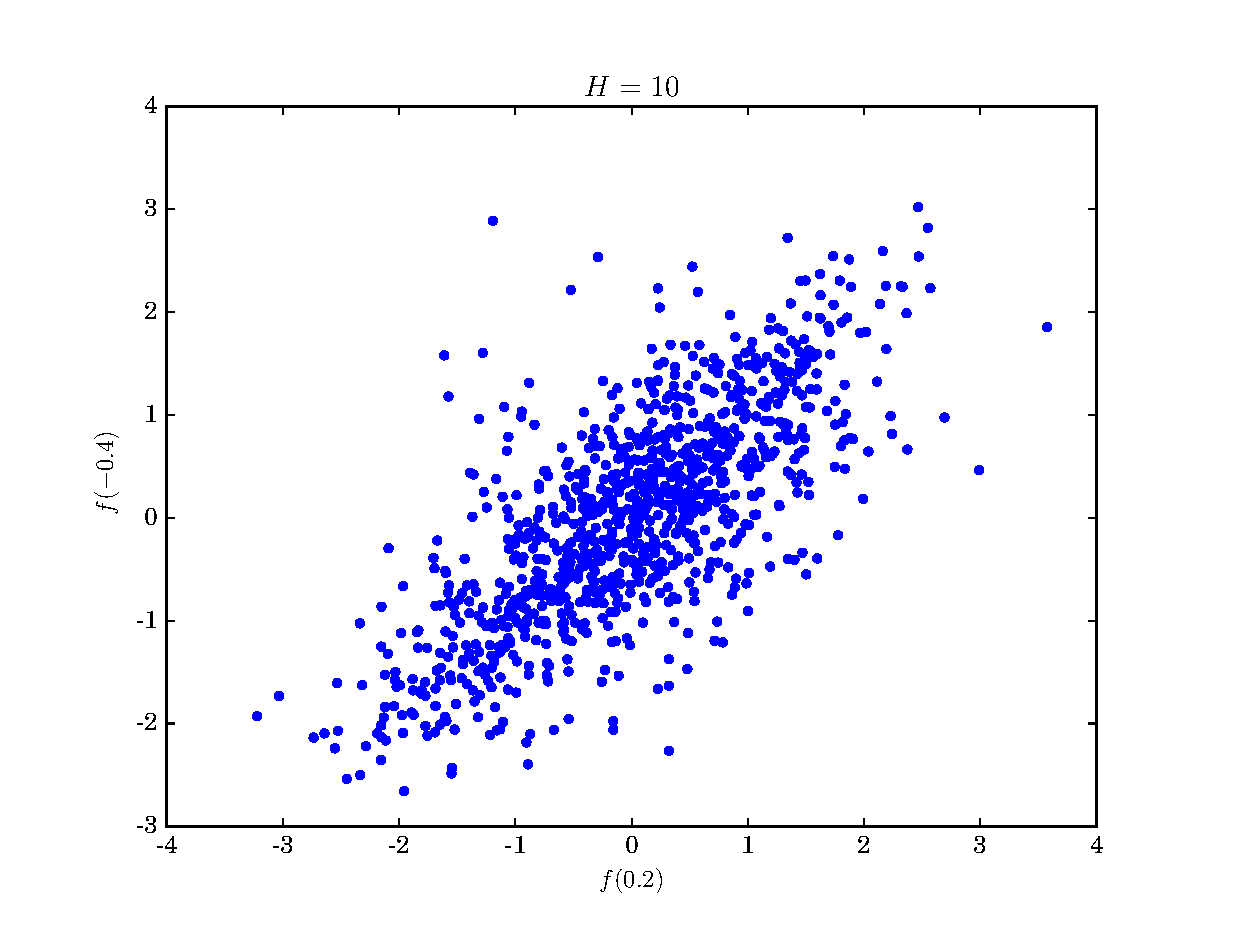
\includegraphics[width=\linewidth]{./figs/10.eps}
      \caption{10 hidden units}
    \end{subfigure}%
    ~ 
    \begin{subfigure}[b]{0.5\textwidth}
      \centering
      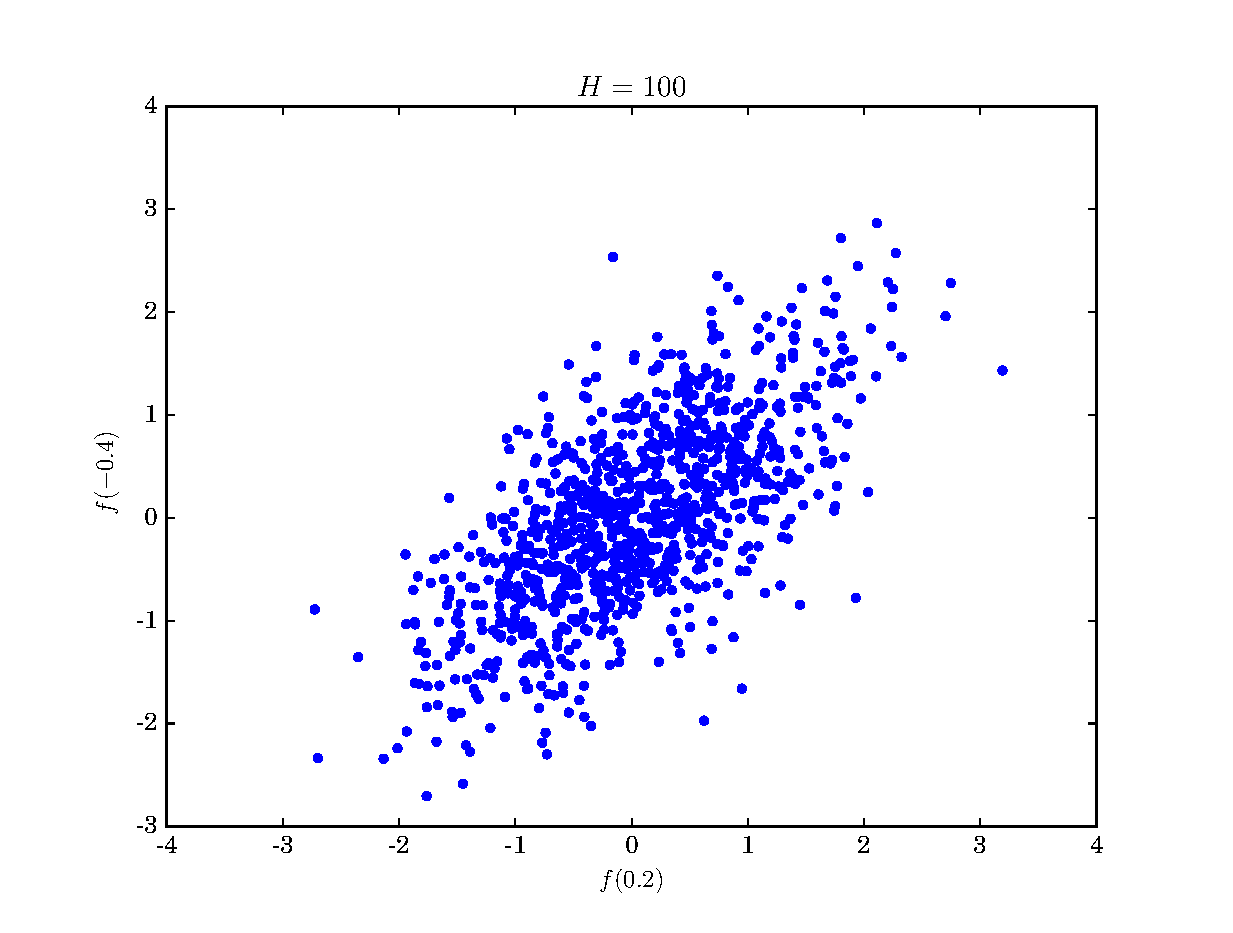
\includegraphics[width=\linewidth]{./figs/100.eps}
      \caption{100 hidden units}
    \end{subfigure}
  \end{figure}
\end{frame}
% 
% 
% 
% 
% ------------------------------------------------
\begin{frame}
  \frametitle{The Bayesian Way}
  Still looking for a for Bayesian treatment of Neural Networks
  \begin{equation*}
    p(\mb{\omega}|\mb{Y}, \mb{X}) = \dfrac{p(\mb{\omega}) p(\mb{Y}|\mb{X}, \mb{\omega})}{p(\mb{Y}|\mb{X})}
  \end{equation*}
  \vspace*{0.5cm}
  \begin{equation*}
    p(\mb{y}^* |\mb{x}^*, \mb{Y}, \mb{X}, \mb{\omega}) = 
    \int p(\mb{y}^* |\mb{x}^*, \mb{\omega}) p(\mb{\omega}|\mb{Y}, \mb{X}) d\mb{\omega}
  \end{equation*}
  %
  %
  But as expected, posterior for a deep neural network is intractable
\end{frame}
% 
% 
% 
% 
% 
% ------------------------------------------------
\begin{frame}
  \frametitle{Current Research}
  \begin{itemize}
  \item Preliminary work done in \cite{Neal1996}, \cite{mackay1992}
    % 
  \item Only recently resurfaced as a topic of interest
    % 
  \item Neural Networks are hard to perform inference on
    % 
  \item Recent work done in \cite{graves2011} is promising to address this issue
    % 
  \item How to use Bayesian methods to model uncertainty in our predictions \cite{kingma2015}, \cite{gal2016}
  \end{itemize}  
\end{frame}
% 
% 
% 
% 
% ------------------------------------------------
\begin{frame}
  \frametitle{Variational Methods}
  Select an approximate posterior $q_\theta(\omega)$ and minimise KL Divergence between approximate and true posterior
  \begin{align*}
    \hat{\mathcal{L}}_{VI}(\theta) &:= - \int q_\theta (\mb{\omega})
    \log\Big( p(\mb{Y} | \mb{X}, \mb{\omega}) \Big) d\mb{\omega} +
    \text{KL}\Big( q_\theta (\mb{\omega}) || p (\mb{\omega}) \Big)
    \\
    \\
                                   &= - \sum_{i=1}^{n_x}\int q_\theta (\mb{\omega})
    \log\Big( p(\mb{y}_i | \mb{f}^{\mb{\omega}}(\mb{x}_i) \Big) d\mb{\omega} +
    \text{KL}\Big( q_\theta (\mb{\omega}) || p (\mb{\omega}) \Big)
  \end{align*}
  First term corresponds to expected log-liklihood
\end{frame}
% 
% 
% 
% 
% ------------------------------------------------
\begin{frame}
  \frametitle{Reparameterisation Trick}
  Expected log-liklihood term is of the form,
  \begin{equation*}
    I(\theta) = \dfrac{\partial}{\partial \theta} \int f(x) p_\theta(x) dx
  \end{equation*}
  We can use the reparameterisation trick proposed in \cite{kingma2013}, where the latent variable $\mb{\omega} \sim q_\theta(\mb{\omega})$ is expressed as a deterministic function $g(\epsilon, \theta)$, with $\mb{\epsilon} \sim p(\mb{\epsilon}) = \Pi_{l,i} p(\epsilon_{l,i})$.
  \\
  \vspace*{0.5cm}
  For example, if $\mb{\omega} \sim \mathcal{N}(\mu, \sigma^2)$, can have $g(\theta, \epsilon) = \mu + \epsilon \sigma$, where $p(\epsilon) = \mathcal{N}(0, I)$
\end{frame}
% 
% 
% 
% 
% 
% ------------------------------------------------
\begin{frame}
  \frametitle{Reparameterisation Trick}
  With this, we can rewrite our KL divergence term between the true and approximate posterior. In this way, our variational objective,
  \begin{equation*}
    \hat{\mathcal{L}}_{VI}(\theta) := - \sum_{i=1}^{n_x}\int q_\theta (\mb{\omega})
    \log\Big( p(\mb{y}_i | \mb{f}^{\mb{\omega}}(\mb{x}_i) \Big) d\mb{\omega} +
    \text{KL}\Big( q_\theta (\mb{\omega}) || p (\mb{\omega}) \Big)
  \end{equation*}
  becomes \cite{gal2016},
  \begin{equation*}
    \hat{\mathcal{L}}_{VI}(\theta) := - \sum_{i=1}^{n_x}\int p(\mb{\epsilon})
    \log\Big( p(\mb{y}_i | \mb{f}^{g(\epsilon, \theta)} (\mb{x}_i) \Big) d\mb{\epsilon} +
    \text{KL}\Big( q_\theta (\mb{\omega}) || p (\mb{\omega}) \Big)
  \end{equation*}  
  This expression can then be approximated using Monte Carlo methods to find our expression for the approximate posterior.
\end{frame}
% 
% 
% 
% 
% 
% ------------------------------------------------
\begin{frame}
  \frametitle{Link to Dropout}
  \begin{equation*}
    \hat{\mathcal{L}}_{VI}(\theta) := - \sum_{i=1}^{n_x}\int p(\mb{\epsilon})
    \log\Big( p(\mb{y}_i | \mb{f}^{g(\epsilon, \theta)} (\mb{x}_i) \Big) d\mb{\epsilon} +
    \text{KL}\Big( q_\theta (\mb{\omega}) || p (\mb{\omega}) \Big)
  \end{equation*}
  In this expression, the term $\mb{f}^{g(\epsilon, \theta)}$ corresponds to the output of the network, with dropout described by $p(\mb{\epsilon}) $ applied to the networks units.

  This expression can then be approximated using Monte Carlo methods to find our expression for the approximate posterior.
  \begin{equation*}
    \hat{\mathcal{L}}_{MC}(\theta) := - \sum_{i=1}^{n_x}
    \log\Big( p(\mb{y}_i | \mb{f}^{g(\hat{\epsilon}, \theta)} (\mb{x}_i) \Big)+
    \text{KL}\Big(q_\theta (\mb{\omega}) || p (\mb{\omega}) \Big)
  \end{equation*}
  This expression can be optimised using gradient descent to optimal parameters $\theta$ for our approximate posterior $q_\theta(\mb{\omega})$.
\end{frame}
% ------------------------------------------------
% 
% 
% 
% 
% ------------------------------------------------
\begin{frame}
  \frametitle{Predictive Posterior}
  \begin{align*}
    \widetilde{\log} \Bigg( p(\mb{y}^* | \mb{x}^*, X, Y) \Bigg)
    &:=  \log \Big(
      \dfrac{1}{T} \sum_{t=1}^T
      p(\mb{y}^* | \mb{x}^*, \mb{\omega}_t) \Big)
    \\
    &\underset{T \rightarrow \infty}{\longrightarrow} \int p(\mb{y}^* | \mb{x}^*, \mb{\omega})
      q_\theta(\mb{\omega}) d\mb{\omega}
    \\
    & \approx \int p(\mb{y}^* | \mb{x}^*, \mb{\omega})
      p(\mb{\omega} | X,Y)  d\mb{\omega}
  \end{align*}
Sampling from this approximate predictive distribution results in multiple forward passes during test time while including stochastic dropout variables \cite{gal2016}.
\end{frame}
% ------------------------------------------------
% 
% 
% 
% 
% ------------------------------------------------

\begin{frame}
  \frametitle{Topics of interest}
  \begin{itemize}
  \item How can we better design neural networks with practical inference in mind
  \item Look at model design, ie. can we let a Bayesian method actually design our model
  \item Bayesian Domain Adaptation: how to use pretrained models as a prior?
  \item Can we incorporate output uncertainty in the training process?
  \item How to make decisions with uncertainty estimations?
  \item How good is our uncertainty estimations?
  \item Big one: How to use a Bayesian framework to better understand deep nets?
  \end{itemize}
\end{frame}
% 
% 
% 
% 
% ------------------------------------------------
\begin{frame}[allowframebreaks]
  \frametitle{References}
  \printbibliography
\end{frame}
%
%
%
%
%----------------------------------------------------------------------------------------
\begin{frame}
  \frametitle{Code}
  Gaussian Process and Neural Network Regression
  \\
  \myhref{https://github.com/ethangoan/regression}{https://github.com/ethangoan/regression}
  \\
  \vspace*{0.5cm}
  Gaussian Prior over model parameters
  \\
  \myhref{https://github.com/ethangoan/bayesian_nn}{https://github.com/ethangoan/bayesian\_nn}
\end{frame}
\end{document}
